\documentclass[10pt,a4paper]{article} %rozmiar czcionki i klasa dokumentu
\usepackage[left=1.5cm, right=1.5cm]{geometry} %szerokosc marginesu
\usepackage[utf8]{inputenc} 
% \usepackage[latin2]{inputenc} ten pakiet gryzie się z powyższym i poniższym!
\usepackage[polish]{babel} %dolacza pakiet z jezykiem polskim 
% \usepackage{polski} alternatywny pakiet
\usepackage[T1]{fontenc} %poprawne składanie polskich czcionek
\usepackage{indentfirst} %pierwszy akapit wciety

\usepackage{graphicx,subfigure}
\usepackage{psfrag}
\usepackage{wrapfig}

\graphicspath{{./obrazki/}}

\usepackage{amsmath}
\usepackage{amsfonts}
\usepackage{array}
\usepackage{supertabular}
\usepackage{array}
\usepackage{tabularx}
\usepackage{hhline}

\usepackage{listings}
\usepackage{xcolor}

\definecolor{codegreen}{rgb}{0,0.6,0}
\definecolor{codegray}{rgb}{0.5,0.5,0.5}
\definecolor{codepurple}{rgb}{0.58,0,0.82}
\definecolor{backcolour}{rgb}{0.95,0.95,0.92}

\lstdefinestyle{selfstyle}{
	backgroundcolor=\color{backcolour},   
	commentstyle=\color{codegreen},
	keywordstyle=\color{magenta},
	numberstyle=\tiny\color{codegray},
	stringstyle=\color{codepurple},
	basicstyle=\ttfamily\footnotesize,
	breakatwhitespace=false,         
	breaklines=true,                 
	captionpos=b,                    
	keepspaces=true,                 
	numbers=left,                    
	numbersep=5pt,                  
	showspaces=false,                
	showstringspaces=false,
	showtabs=false,                  
	tabsize=2
}

\lstset{style=selfstyle}
\begin{document}
\title{PAMSI - Projekt nr.3 \\
	   \large Grafy}
\author{Dawid Krekora 254003}
\date{\today}
\maketitle
\tableofcontents
	\newpage
	\section{Wprowadzenie}
	Zadanie projektowe polegało na napisaniu dwóch implementacji grafów:
	\begin{itemize}
		\item Za pomocą listy sąsiedztwa
		\item Za pomocą macierzy sąsiedztwa
	\end{itemize} 
	Następnie należało zaimplementować dwa algorytmy operujące na grafach, zajmujące się problemami znajdowania najkrótszej ścieżki w grafie. Algorytmy te zostały poddane testowi efektywności w zależności od gestości grafu oraz ilości krawędzi. Grafy które zostały poddane testom były grafami ważonymi, skierowanymi.
	\section{Opis badanych algorytmów}
	W zadaniu projektowym poddano badaniom dwa algorytmy wyszukiwania najkrótszej ścieżki. Algorytmy te zostały bliżej przedstawione poniżej.
	\subsection{Algorytm Dijkstry}
	Algorytm Dijkstry jest najpopularniejszym algorytmem (ma szerokie spektrum zastosowań) zajmującym się badaniem problemu najkrótszej drogi. Spowodowane jest to głównie jego efektywnością działania. Szacuje się, że złożoność obliczeniowa algorytmu Dijkstry wynosi $\textbf{O}(Elog_{V}$) gdzie:
	\begin{itemize}
		\item E - liczba krawędzi grafu
		\item V - liczba wierzchołków w grafie
	\end{itemize}
	Wymieniona złożoność dotyczy implementacji tablicy kosztów dojścia do wierzchołków w postaci kolejki priorytetowej. W naszym przypadku użyto zwykłej iteracji tablicowej która jest mniej efektywna. Działanie algorytmu Dijkstry opiera się zależnościach między  wierzchołkami incydentnymi aktualizując w każdej iteracji drogę potrzebną do dotarcia do sąsiadów wybranego wierzchołka. Sam wierzchołek natomiast jest przenoszony do zbioru wierzchołków przetworzonych. Dzieje się tak do momentu aż wszystkie wierzchołki nie zostaną przetworzone.
	\subsection{Algorytm Bellmana-Forda}
	Algorytm Bellmana-Forda posiada podobne działanie do algorytmu Dijkstry - podobne dlatego, że również możemy za jego pomocą znaleźć drogę do wszystkich wierzchołków i określić jej koszt dojścia. W praktyce jednak rozszerza nam działanie algorytmu Dijstry ponieważ jest w stanie wykryć negatywne cykle (cykle w których wraz z każdym przejściem koszt dojścia do wierzchołka maleje), które fałszują wyniki końcowe. W takim przypadku algorytm wykryje taką nieprawidłowość i nas o tym poinformuje. Niestety funkcjonalność ta jest obarczona dodatkową złożonością obliczeniową która szacowana jest na $\textbf{O}(E*V$). Wynika to przede wszystkim z konieczności sprawdzania wszystkich krawędzi grafu w każdej z iteracji (których suma jest nie mniejsza niż całkowita liczba wierzchołków w grafie). Jeżeli zostanie wykryty negatywny cykl algorytm zwróci wartość 1. Natomiast w przypadku poprawnego grafu wartość 0, co oznacza paradoksalnie: wszystko jest poprawne, nie wykryto (wartość 0) negatywnych cykli. Następnie uzyskamy rezultat działań identyczny z algorytmem Dijkstry.
	\clearpage
	\section{Przebieg eksperymentów}
	Do eksperymentów użyto funkcjonalność bibloteki \textit{chrono} z pakietu biblotek C++. Dla każdej ilości wierzchołków (10,50,100,150,200) i każdej gęstości grafu (0.25,0.5,0.75,1) wywołano 100 losowych instancji grafów ważonych, skierowanych. Czas działania każdej instancji dla każdego testu (łącznie 20 testów) zarejestrowano za pomocą wspomnianej wcześniej bibloteki, dodano całowity przebieg czasowy, a następnie określono wartość średnią dla każdego testu. Wyniki przedstawione w tabeli (rys.1) zostały naniesione według różnych kryteriów zawartych w tytułach wykresów (rys.2-7).
	\begin{figure}[!ht]
		\centering %centruje obrazek na stronie 
		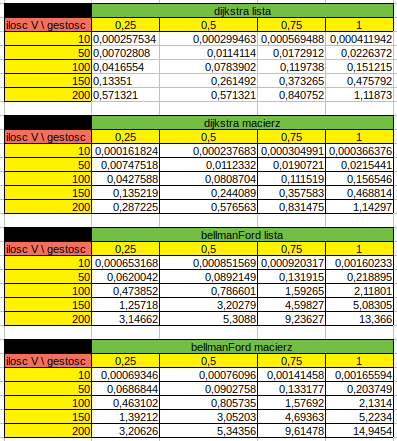
\includegraphics[scale = 0.9]{tabela.png} %Skaluje obrazek mnożąc jego wymiary przez podaną liczbę.
		\caption{Tabela wyników czasu działania algorytmów (wartości średnie)} %dodaje opis do obrazka
		\label{fig:Obraz1} %Tworzy odnośnik do obrazka
	\end{figure}

	\clearpage
	
	\begin{figure}[!ht]
		\centering %centruje obrazek na stronie 
		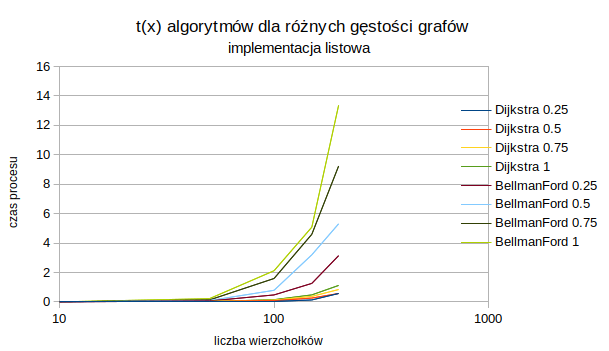
\includegraphics[scale = 0.9]{dijstra_bellman_lista.png} %Skaluje obrazek mnożąc jego wymiary przez podaną liczbę.
		\caption{Funkcja czasu działania algorytmu od ilości jego wierzchołków - implementacja listowa} %dodaje opis do obrazk
		\label{fig:Obraz2} %Tworzy odnośnik do obrazka
	\end{figure}
	\begin{figure}[!ht]
		\centering %centruje obrazek na stronie 
		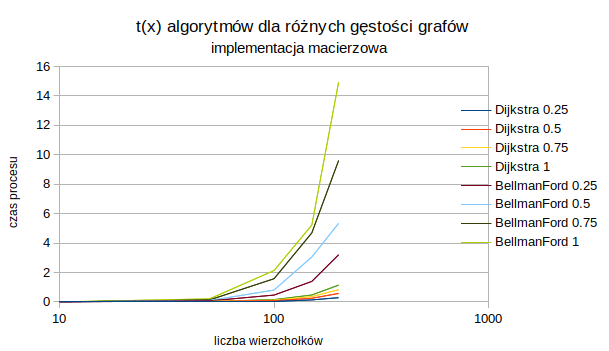
\includegraphics[scale = 0.9]{dijstra_bellman_macierz.png} %Skaluje obrazek mnożąc jego wymiary przez podaną liczbę.
		\caption{Funkcja czasu działania algorytmu od ilości jego wierzchołków - implementacja macierzowa} %dodaje opis do obrazka
		\label{fig:Obraz3} %Tworzy odnośnik do obrazka
	\end{figure}
	
	\clearpage
	
	\begin{figure}[!ht]
		\centering %centruje obrazek na stronie 
		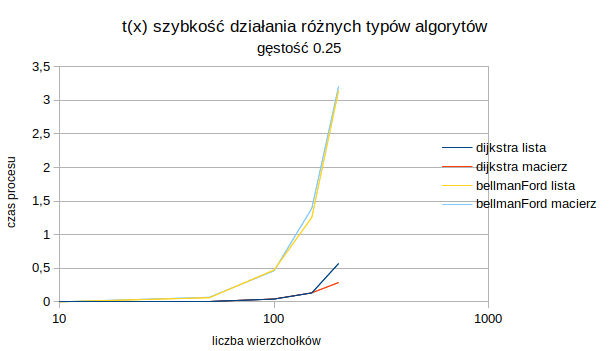
\includegraphics[scale = 0.9]{dijkstra_bellman_gestosc025.png} %Skaluje obrazek mnożąc jego wymiary przez podaną liczbę.
		\caption{Funkcja czasu działania algorytmu od ilości jego wierzchołków - gestość 0.25 dla różnych implementacji} %dodaje opis do obrazk
		\label{fig:Obraz4} %Tworzy odnośnik do obrazka
	\end{figure}
	\begin{figure}[!ht]
		\centering %centruje obrazek na stronie 
		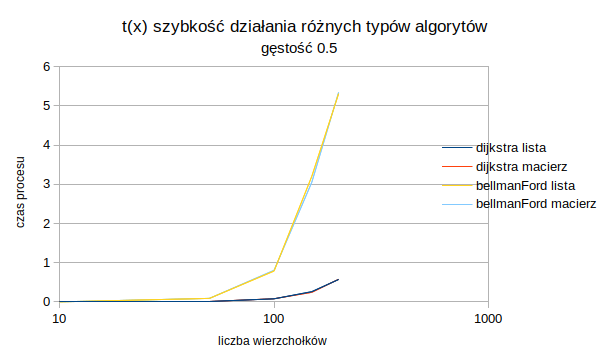
\includegraphics[scale = 0.9]{dijkstra_bellman_gestosc05.png} %Skaluje obrazek mnożąc jego wymiary przez podaną liczbę.
		\caption{Funkcja czasu działania algorytmu od ilości jego wierzchołków - gestość 0.5 dla różnych implementacji} %dodaje opis do obrazka
		\label{fig:Obraz5} %Tworzy odnośnik do obrazka
	\end{figure}

	\clearpage
	
	\begin{figure}[!ht]
		\centering %centruje obrazek na stronie 
		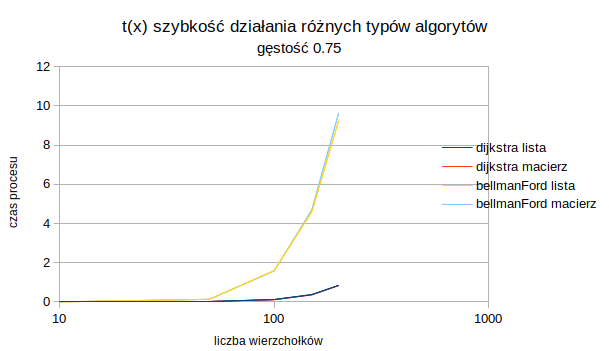
\includegraphics[scale = 0.9]{dijkstra_bellman_gestosc075.png} %Skaluje obrazek mnożąc jego wymiary przez podaną liczbę.
		\caption{Funkcja czasu działania algorytmu od ilości jego wierzchołków - gestość 0.75 dla różnych implementacji} %dodaje opis do obrazk
		\label{fig:Obraz6} %Tworzy odnośnik do obrazka
	\end{figure}
	\begin{figure}[!ht]
		\centering %centruje obrazek na stronie 
		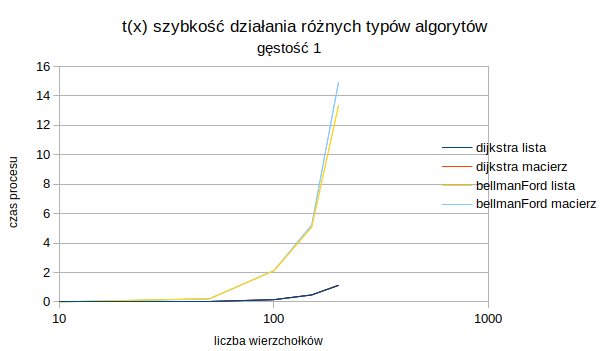
\includegraphics[scale = 0.9]{dijkstra_bellman_gestosc1.png} %Skaluje obrazek mnożąc jego wymiary przez podaną liczbę.
		\caption{Funkcja czasu działania algorytmu od ilości jego wierzchołków - gestość 1 dla różnych implementacji} %dodaje opis do obrazka
		\label{fig:Obraz7} %Tworzy odnośnik do obrazka
	\end{figure}
	
	\section{Podsumowanie i wnioski}
	\begin{itemize}
		\item Czas działania algorytmów był zgodny z naszymi założeniami. Dla małej ilości wierzchołków nie miała znaczenia ani gęstość grafu, ani sposób jego implementacji. 
		\item Wraz ze wzrostem liczby wierzchołków można było zauważyć znaczące różnice w długości działania. Algorytm Bellmana-Forda okazał się niezwykle konsumpcyjny. Dla maksymalnych gęstości czas jego działania był ponad 10 krotnie większy od czasu działania algorytmu Dijkstry. Sposób implementacji nie miał w tym wypadku większego znaczenia (różnice czasowe były niewielkie - na korzyść w jedną lub drugą stronę). Z najbardziej złożonym problemem najlepiej poradziła sobie implementacja listowa.
		\item Zdecydowania lepszym algorytmem znajdowania najkrótszej ścieżki okazał się algorytm Dijkstry i to on jest używany w przytłaczającej przewadze nad algorytmem Bellmana-Forda. Wynika to z faktu, że rzadko mamy do czynienia z reprezentacją danych w której występuje negatywny cykl. Zwycięski algorytm znalazł zastosowanie m.in. w wyznaczaniu drogi na mapie - oczywiście z nieco efektywniejszej formie. 
	\end{itemize}
	\section{Bibliografia}
	\begin{itemize}
		\item Piotr Wróblewski, W: Helion, "Algorytmy, struktury danych i techniki programowania", 2009
		\item https://baeldung.com/cs/bellman-ford
		\item https://eduinf.waw.pl/inf/alg/001 search/index.php
		\item Michael T.G,Roberto T., David M.,W: John Wiley and Sons Inc. , "Data structures and algorithms in $C++$", 2009 	
\end{itemize}

		
\end{document}